\section{The LSST Camera (LSSTCam)} \label{sec:lsstcam}

% Biblio
The Vera C. Rubin Observatory's camera LSSTCam \cite{10.71929/rubin/2571927} is the largest digital camera ever built to date.
Its design, and the technical progress it demanded, were developed in order to meet the requirements set by the ambitious goals of LSST, as described in \cite{2024SPIE13096E..1SR}.
We have thus created an ISR approach specifically for the analysis of LSSTCam images.
Figure \ref{fig:beforeafterISR} shows an example of the results from our ISR pipeline on an LSSTCam exposure, showing the corrections of large effects (such as the amplifier offset or crosstalk)
as well as more subtle effects (such as the brighter fatter effect) described in details in following sections.
We summarize here key points about LSSTCam and properties of its CCDs relevant to LSSTCam calibration in Rubin Data Management (DM).

\begin{figure*}[t]
    \centering
    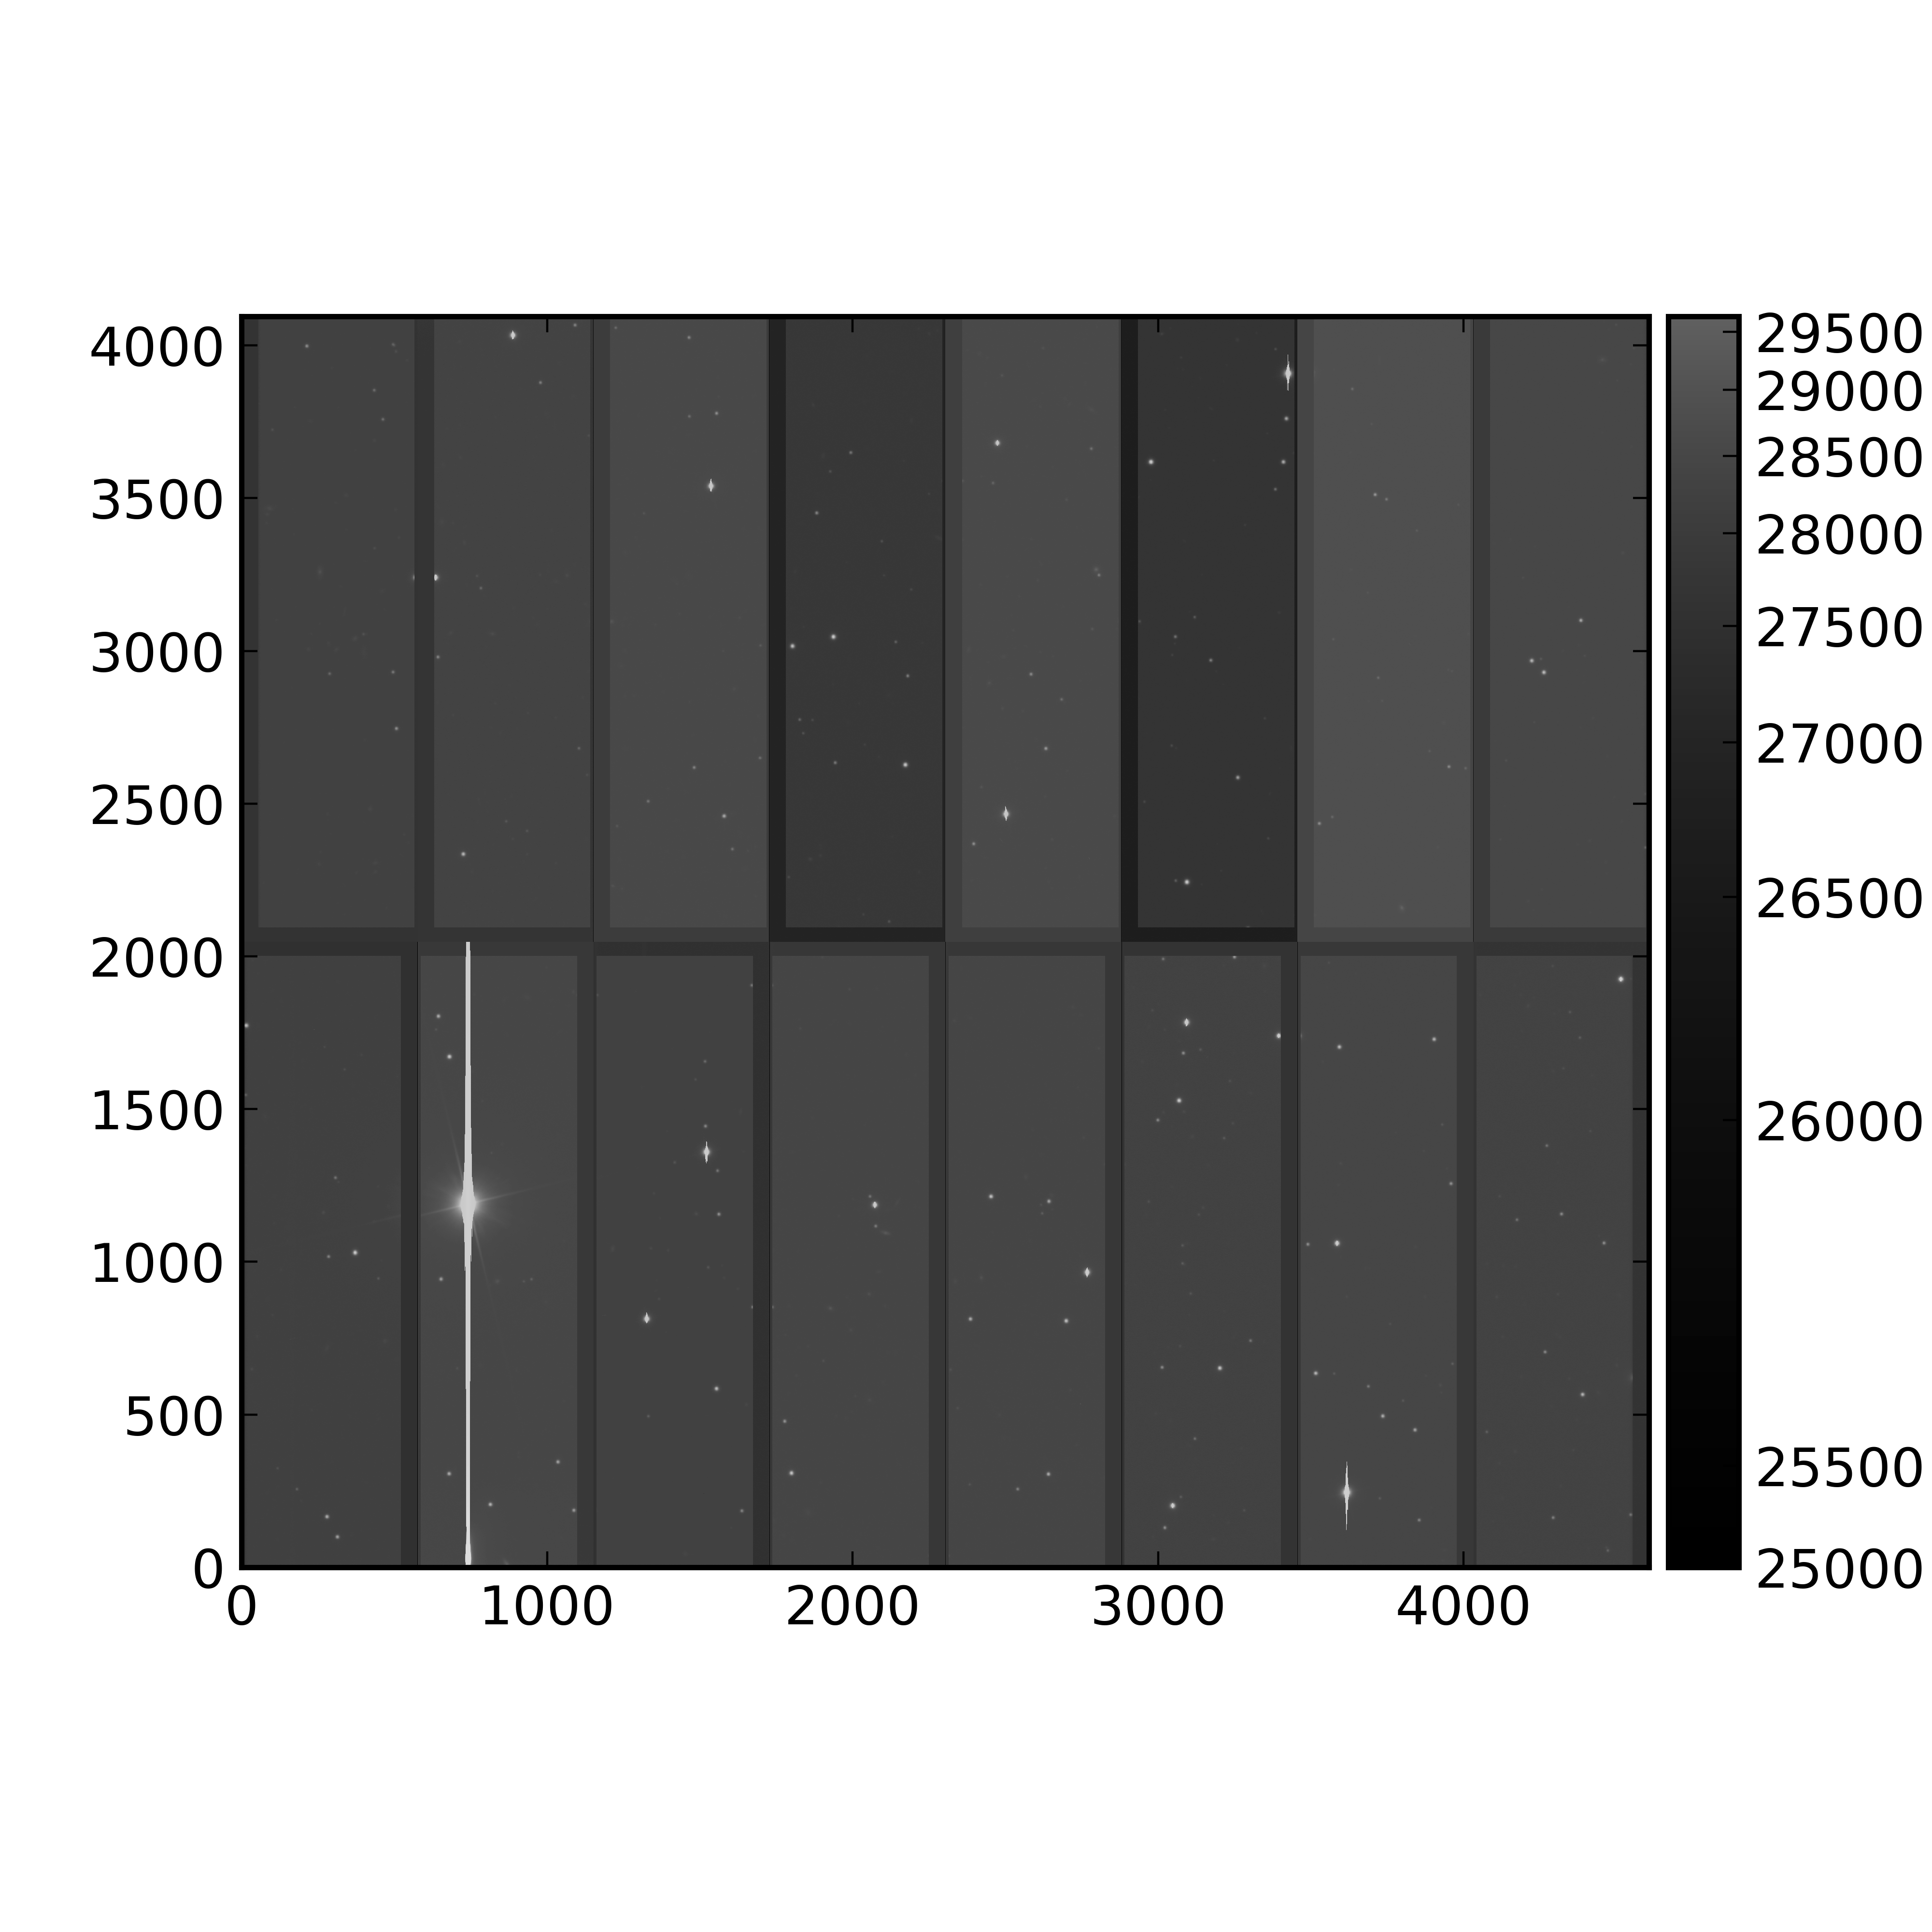
\includegraphics[width=0.4\textwidth]{figures/2026010700083_81_beforeISR.png}
    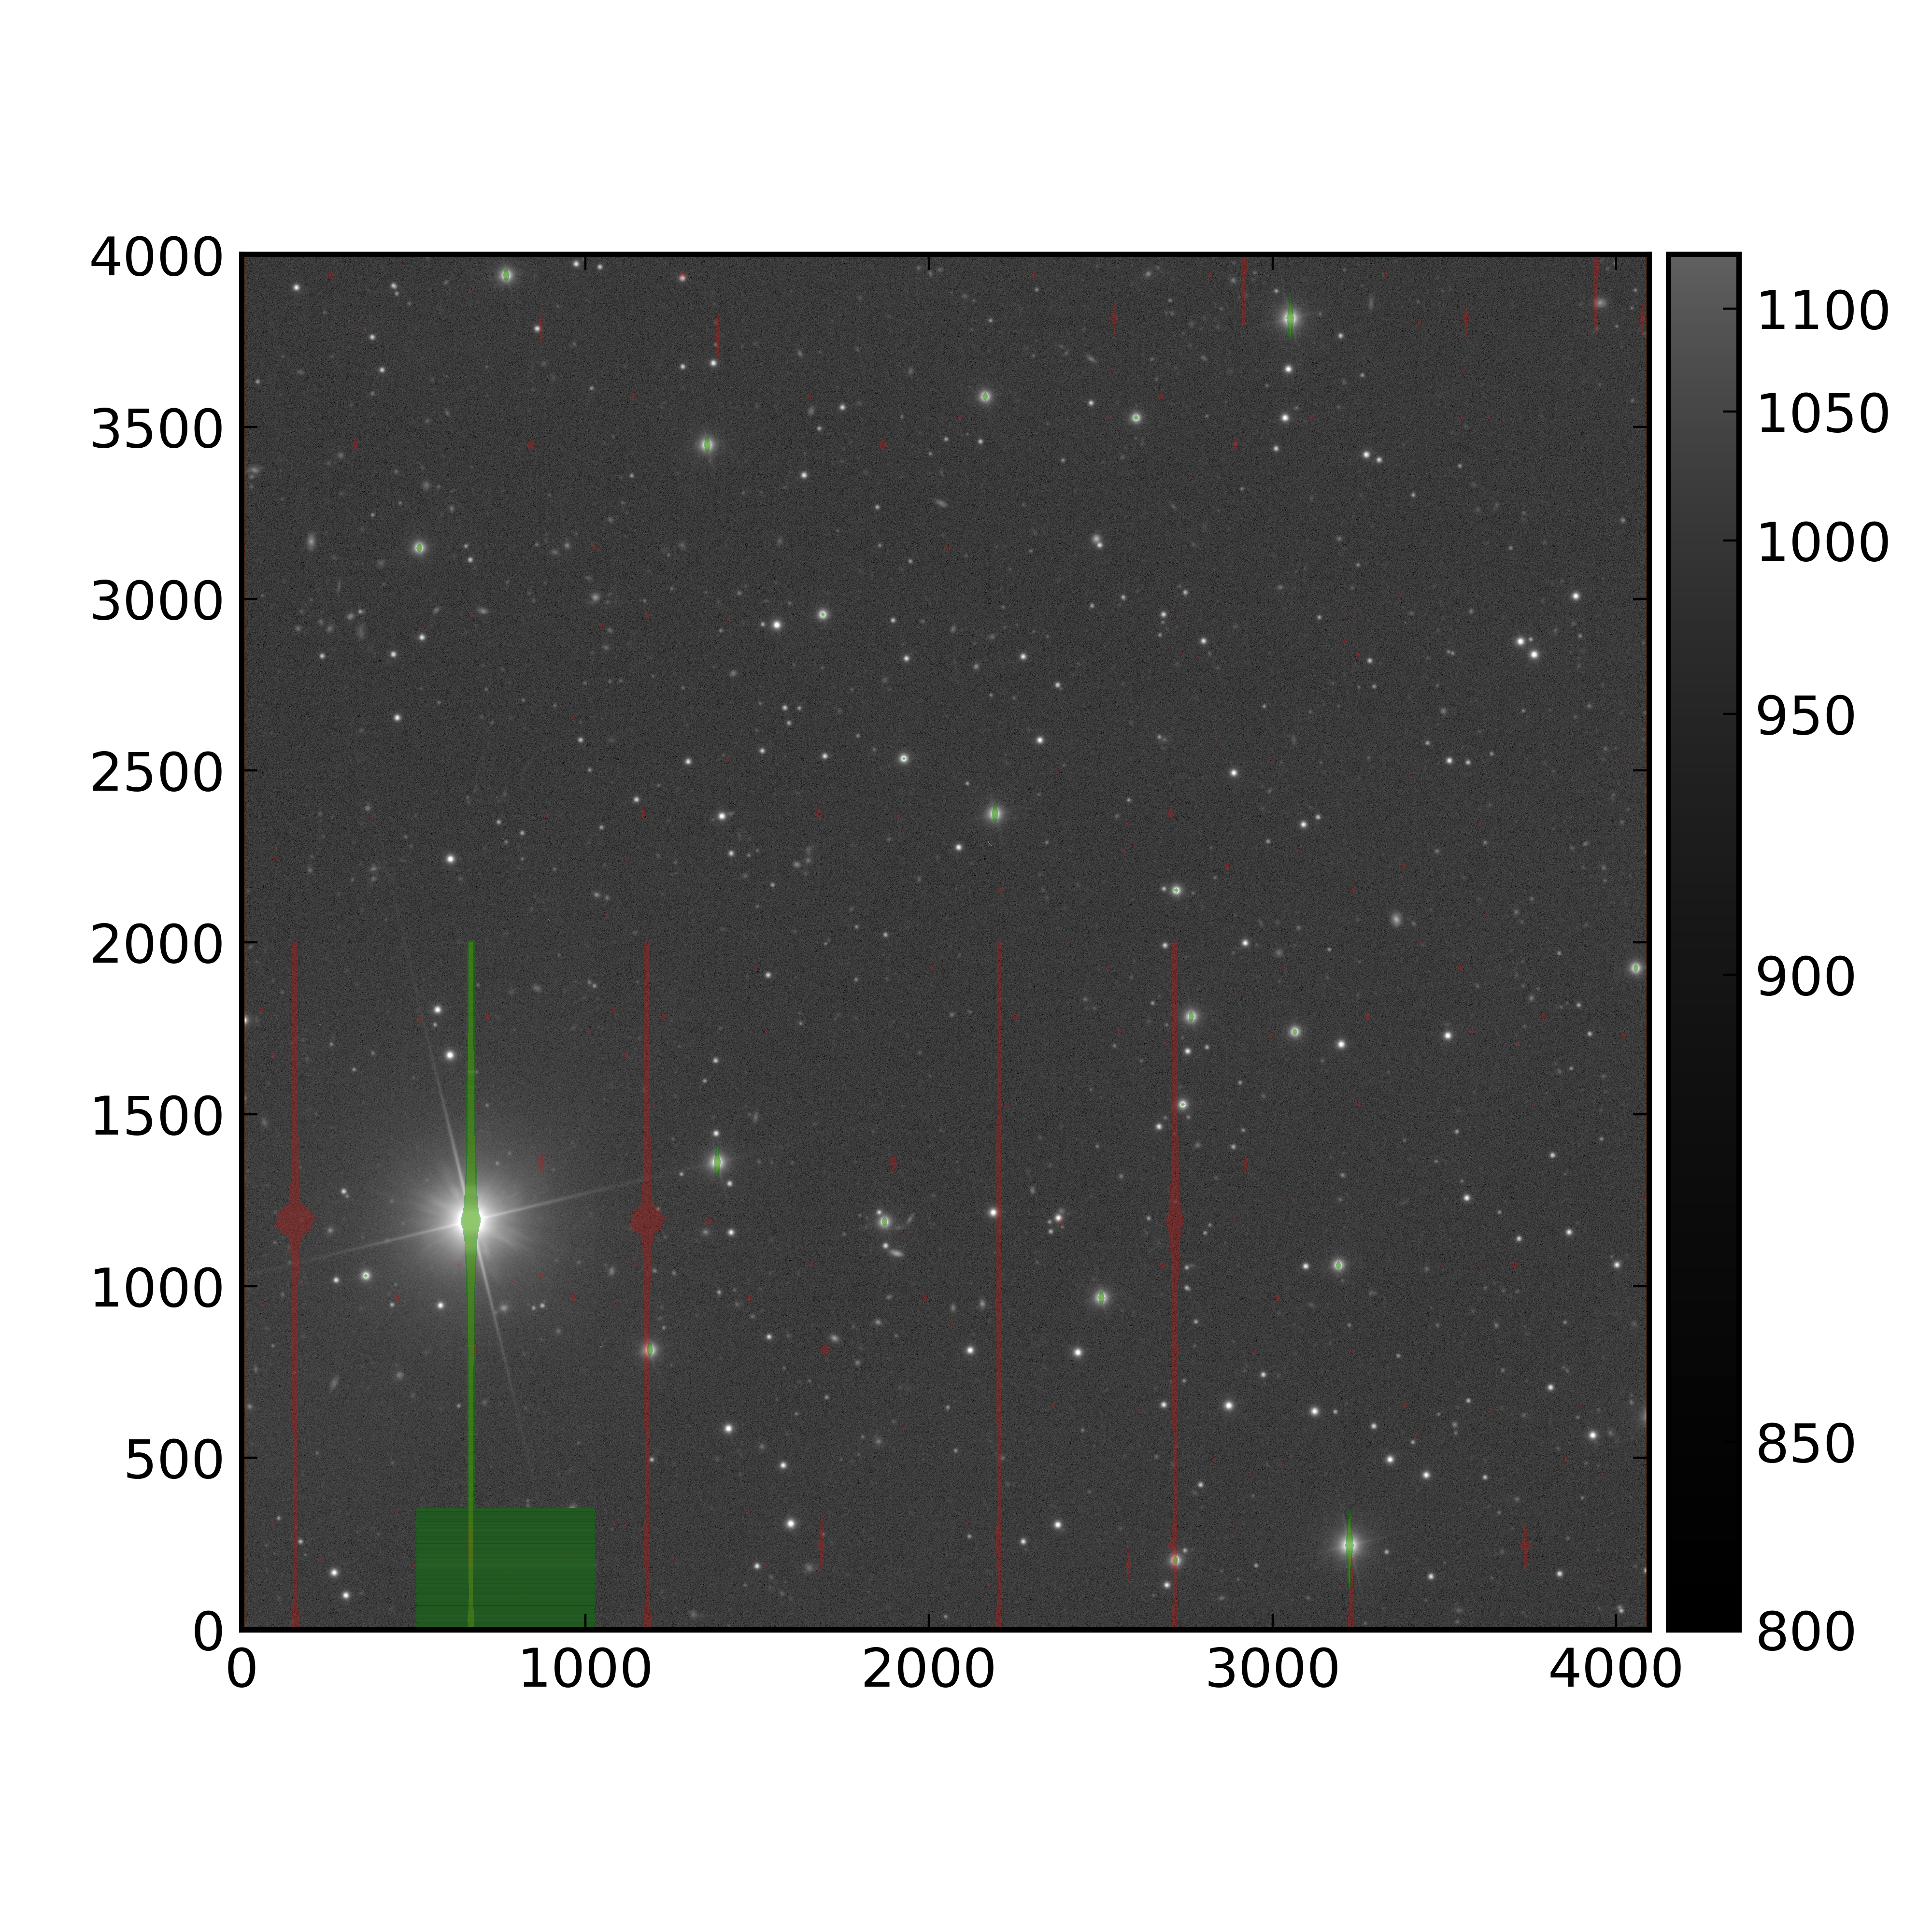
\includegraphics[width=0.4\textwidth]{figures/2026010700083_81_afterISR.png}
    \caption{The left panel shows a raw image of detector 81 (e2v type) of exposure 2026010700083,
    and the right panel shows the resulting image from processing it through the DP2 ISR pipeline.
    Some corrections operated by ISR are visually noticable such as a saturation and edge bleed masking (green mask),
    detector assembly,and crosstalk masking (red mask on the right).
    }
    \label{fig:beforeafterISR}
\end{figure*}


\subsection{LSSTCam CCDs} \label{sec:lsstcam:ccds}

% Focal plane
LSSTCam is composed of 189 science CCDs organized in rafts of 9 CCDs (3x3), in a focal plane mosaic presented in \citet{CTN-001}.
Each raft is composed of 3 Readout Electornics Boards (REB) providing the electronics of three neighboring CCDs.
In addition, 2 star guider CCDs and one split-wavefront CCD are at each four corners of the focal plane mosaic.
We will focus only on the science CCDs in the following as no requirements are set on the calibration of the corner sensors within DM, although some calibrations are provided for the star guiders.

% CCDs
LSSTCam CCDs are made of 16 segments each, 8 at the top and 8 at the bottom of the CCD, read out through an amplifier.
Segments are commonly referred to as amplifiers and will be in the rest of this paper.
Each amplifier is 2048 pixels high and 512 pixels wide for e2v and 2048 pixels high and 576 pixels wide for ITL.
Figure \ref{fig:amplifier} shows a diagram of the amplifier geometry and direction of electrons transportation in LSSTCam CCDs.
%here add more about electron transportation and size of ovescan region and serial register.
The overscan regions are virtual pixels read to estimate charge transfer inefficiency (CTI), see \ref{sec:processing:calibration:cti} for my details.
Figure \ref{fig:amplifier} show an example of the signal read in the overscan region for ITL and e2v amplifiers.

\begin{figure*}[t]
    \centering
    % TODO: add amplifier geometry figure asset
    \fbox{\parbox{0.75\textwidth}{\centering\vspace{1.5in}\small\textit{Figure pending}\vspace{1.5in}}}
    \caption{Here is an exposure in e2v amplifier and in ITL amplifier with rectangles around different regions (overscans, serial register)
    and graphs of the signal in their overscan regions.
    }
    \label{fig:amplifier}
\end{figure*}


\subsection{Electronic Detector Model for LSSTCam} \label{sec:lsstcam:detector-model}\label{sec:processing}


The calibration and instrument signature removal (ISR) pipeline removes instrumental effects from science data.
For each effect observed in LSSTCam, the Rubin Science Pipelines define a calibration-generation task that produces the corresponding data product, and a correction task that applies that product during ISR.
We have built on the ISR approach of past optical surveys \textcolor{red}{here add citations for ISR procedures for other CCD optical experiments}
to develop an ISR pipeline specifically designed for LSSTCam.
We have defined the electronic model of LSSTCam and associated effects in the photon to ADU signal chain.
Figure \ref{fig:detector-boxes} depicts the different steps in this chain and their physical ordering from the detector
to the Readout Board (REB). \textcolor{red}{here add any citations that supports this description.}

Calibration and ISR tasks are organized as a pipeline based on our current model of the detector physics.
The calibration production tasks are run in chronological order with respect to the photon transfer and data-acquisition chain, and ISR correction tasks are applied in the opposite order to the sequence in which effects accumulate along the signal path.

The algorithms and processing steps required for LSSTCam calibration and ISR were developed from measurements and analysis during electro-optical testing on the laboratory test stand at SLAC National Accelerator Laboratory, at the summit, and on the telescope in-dome during commissioning.
\citet{2024SPIE13096E..1SR} gives a detailed account of system characterization work and results from the laboratory campaigns.
Figure~\ref{fig:detector-boxes} summarizes the instrumental effects identified in the photon transfer chain and their order.

\begin{figure*}[t]
    \centering
    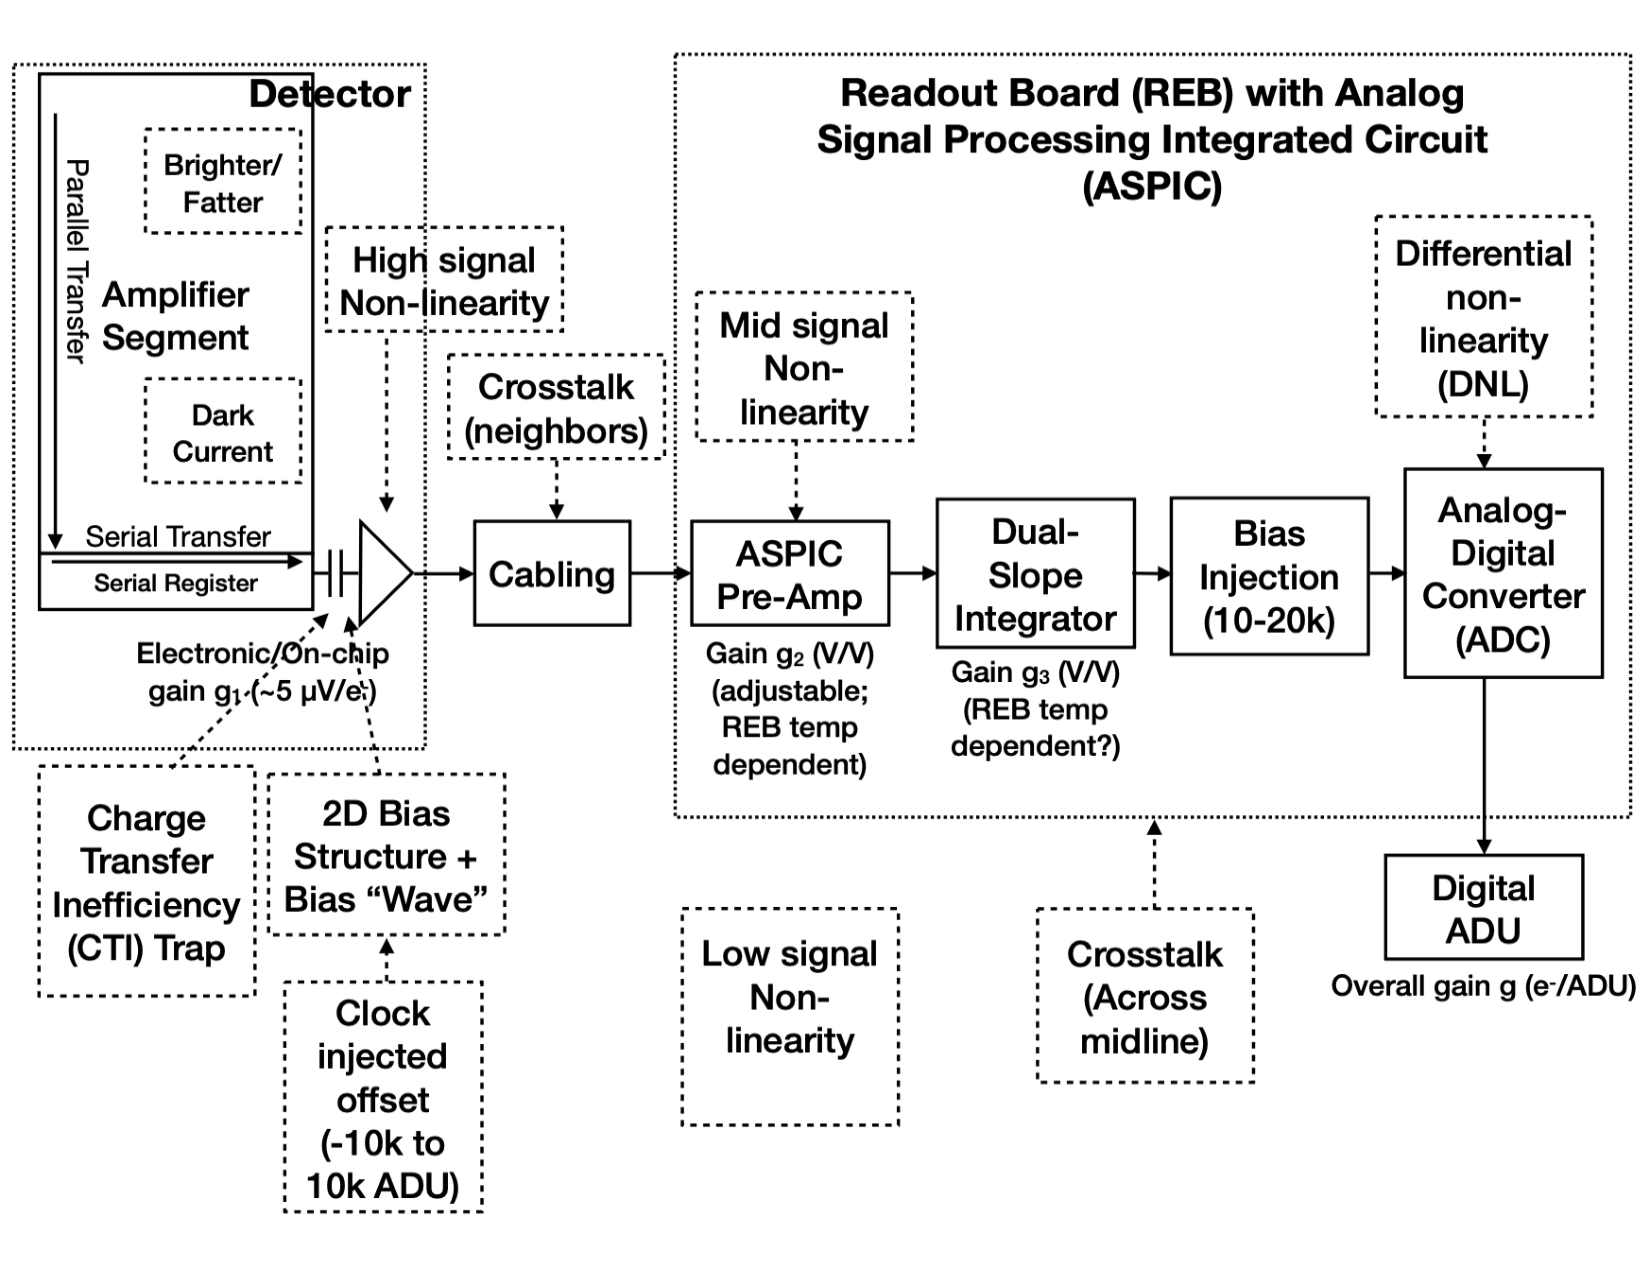
\includegraphics[width=0.8\textwidth]{figures/calibration_boxes_detector_model.pdf}
    \caption{Photon transfer and data-acquisition model for the LSSTCam detectors and electronic readout board (REB).
    Instrumental effects seen in images are shown as dashed boxes; arrows indicate where each effect enters the chain.
    Low-signal nonlinearities in LSSTCam's detector response have been observed, but their origin is not yet established; that contribution appears as a disconnected box.}
    \label{fig:detector-boxes}
\end{figure*}


%Figure~\ref{fig:detector-boxes} summarizes the instrumental effects identified in the photon transfer chain and their order.

%The ISR pipeline implemented in the Rubin data processing aims at correcting each of these effects in the order opposite to which they happen.
